\subsection{Les Tests}

\begin{frame}{Nos réalisations}{Tests}
	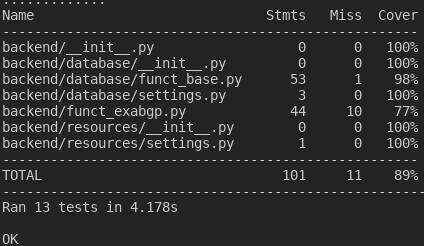
\includegraphics[width=\textwidth]{backend_coverage_v2.png}
\end{frame}

\begin{frame}[fragile]{Nos réalisations}{Tests}
    \begin{minipage}{0.3\textwidth}
        \begin{minted}{python}
           @patch('backend.funct_exabgp.requests.post')
            def test_action_when_command_not_good(self, mock_post):
                 mock_post.return_value.ok = False
                    cmd = [
                        'toto',
                        '',
                        'fj',
                        'help',
                        'kqslfqlsfpaoi)é65eze5a6e5zae6',
                    ]
                    for cmd in self.exabgp_cmd:
                        response = self.exabgp.action(cmd)
                        self.assertIsNone(response)
        \end{minted}
    \end{minipage}
\end{frame}

\begin{frame}{Nos réalisations}{Tests}
    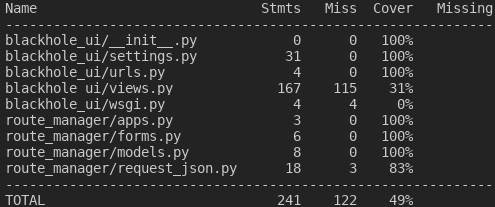
\includegraphics[width=\textwidth]{frontend_coverage_v2.png}
\end{frame}

\begin{frame}{Nos réalisations}{Performance}
    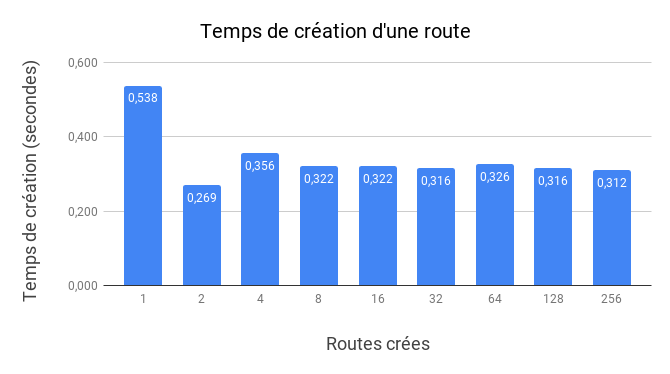
\includegraphics[width=\textwidth]{creation_route_time.png}
\end{frame}

\begin{frame}{Nos réalisations}{Performance}
    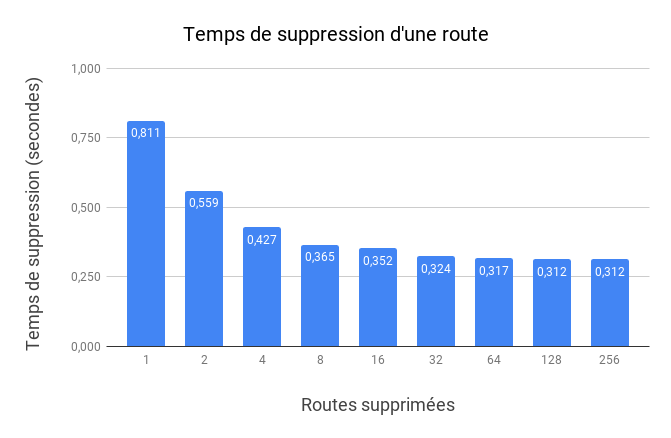
\includegraphics[width=\textwidth]{deletion_route_time.png}
\end{frame}

\begin{frame}{Nos réalisations}{Performance}
    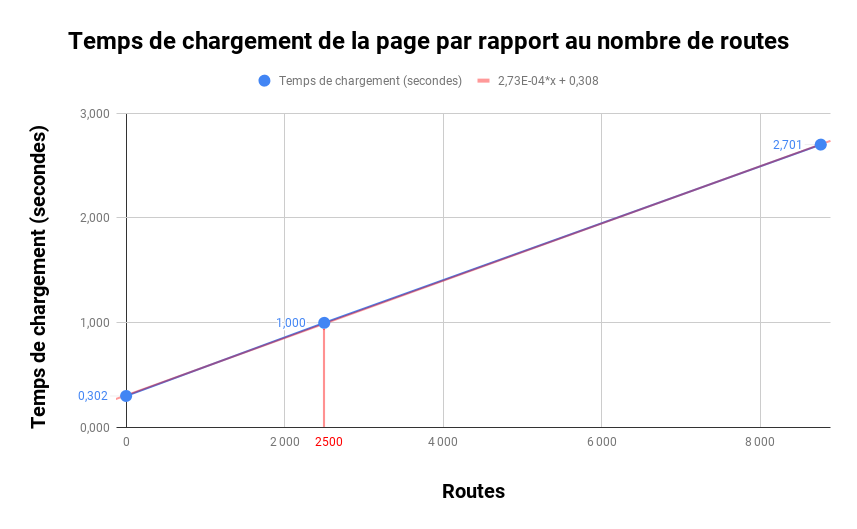
\includegraphics[width=\textwidth]{small_scale.png}
\end{frame}

\begin{frame}{Nos réalisations}{Performance}
    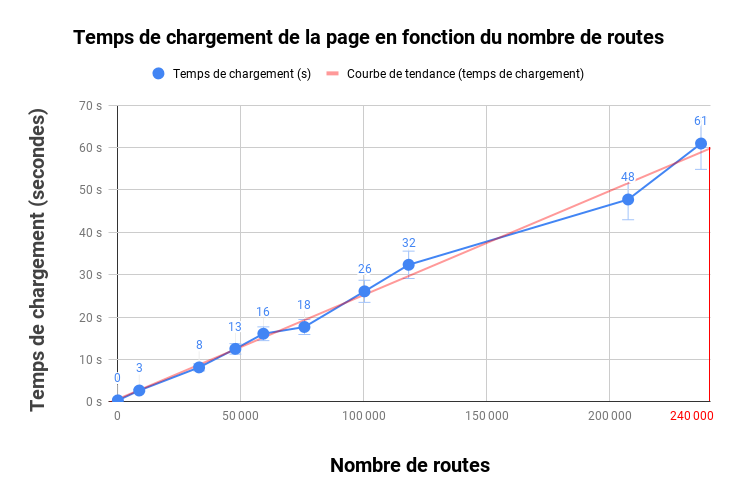
\includegraphics[width=\textwidth]{big_scale.png}
\end{frame}